%%%%%%%%%%%%%%%%%%%%%%%%%%%%%%%%%%%%%%%%%%%%%%%%%%%%
%\graphicspath{chapters/figures/}
\section{Memory Stage}
\label{chap_mem}
%%%%%%%%%%%%%%%%%%%%%%%%%%%%%%%%%%%%%%%%%%%%%%%%%%%%%%%%%%%
This stage can be divided in two major parts: the registers that contains the addresses and the data to be written in the memory or read from the memory and the RAM. The former is actually embedded in the processor, while the latter one is actually external, but provides an interface and some signals to communicate with the processor itself. 
\subsection{Embedded part}
The part included in the datapath is mainly made up of three different registers, which are used to store different values coming from different units:
\begin{itemize}
	\item \textit{dest\_reg}, which is used to save the address of the commit register, to be passed to the following write back stage
	\item \textit{mem\_reg}, where the data coming from the external memory presented in \ref{ram} are stored 
	\item \textit{exec\_reg}, which is used to save the address of the commit register, to be passed to the following write back stage
\end{itemize}
All these registers share the same reset, clock and enable signals. They differ for the input/output ones, which are summarized in table \ref{reg_table}.

\begin{table}[]
	\centering
	\begin{tabular}{llll}
		\toprule
		Reg Name  & \#  bits & Input     & Output   \\
		\midrule
		exec\_reg & 32       & FROM\_ALU & ALU\_OUT  \\
		mem\_reg  & 32       & FROM\_MEM & MEM\_OUT  \\
		dest\_reg & 5        & DEST\_IN  & DEST\_OUT \\
		\bottomrule
	\end{tabular}
	\caption{Table with registers of Memory Stage}
	\label{reg_table}
\end{table}

\subsection{External RAM}
\label{ram}
The external RAM receives signals both from the datapath and from the CU. An overview can be seen in figure \ref{ext_ram_fig}. This part is external since it will not be synthesized. In particular, here are presented the most relevant ones:
\begin{itemize}
	\item \textit{WR} is a signal used to control the writing on the memory.It 
	si intended as active high to complete a write
	\item \textit{D\_TYPE} specifies the kind of data we are reading or writing in/from memory, i.e byte, half-word, word
	\item \textit{US} defines a signed/unsigned representation for the data; it is relevant to correctly extend the data on 32 bits
	\item \textit{ADDRESS} obviously used to correctly point to a precise memory location
	\item \textit{MEMIN} is the signal containing values to be eventually stored in memory
	\item \textit{MEMOUT} is the output signal which cotains the data read from the memory
\end{itemize}

While the writing is performed synchronously only if the \textit{WR} signal is 
high, there is always a value in correspondence of the output signal. This 
means that a read always happens, and a value is written every time on the 
\textit{MEMOUT} signal. This value will be eventually discarded in the 
following stages.

\begin{figure}
	\centering
	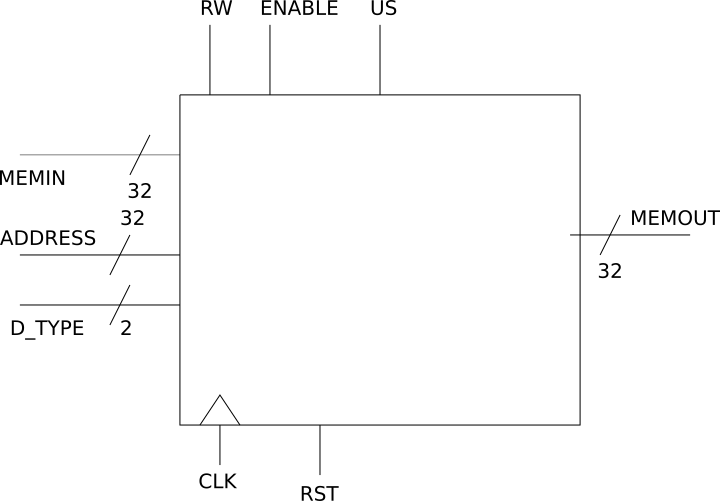
\includegraphics[scale=0.5]{chapters/figures/ram_ext}
	\caption{Interface for external RAM}
	\label{ext_ram_fig}
\end{figure} 
